\documentclass[color=usenames,dvipsnames]{beamer}\usepackage[]{graphicx}\usepackage[]{color}
% maxwidth is the original width if it is less than linewidth
% otherwise use linewidth (to make sure the graphics do not exceed the margin)
\makeatletter
\def\maxwidth{ %
  \ifdim\Gin@nat@width>\linewidth
    \linewidth
  \else
    \Gin@nat@width
  \fi
}
\makeatother

\definecolor{fgcolor}{rgb}{0, 0, 0}
\newcommand{\hlnum}[1]{\textcolor[rgb]{0.69,0.494,0}{#1}}%
\newcommand{\hlstr}[1]{\textcolor[rgb]{0.749,0.012,0.012}{#1}}%
\newcommand{\hlcom}[1]{\textcolor[rgb]{0.514,0.506,0.514}{\textit{#1}}}%
\newcommand{\hlopt}[1]{\textcolor[rgb]{0,0,0}{#1}}%
\newcommand{\hlstd}[1]{\textcolor[rgb]{0,0,0}{#1}}%
\newcommand{\hlkwa}[1]{\textcolor[rgb]{0,0,0}{\textbf{#1}}}%
\newcommand{\hlkwb}[1]{\textcolor[rgb]{0,0.341,0.682}{#1}}%
\newcommand{\hlkwc}[1]{\textcolor[rgb]{0,0,0}{\textbf{#1}}}%
\newcommand{\hlkwd}[1]{\textcolor[rgb]{0.004,0.004,0.506}{#1}}%
\let\hlipl\hlkwb

\usepackage{framed}
\makeatletter
\newenvironment{kframe}{%
 \def\at@end@of@kframe{}%
 \ifinner\ifhmode%
  \def\at@end@of@kframe{\end{minipage}}%
  \begin{minipage}{\columnwidth}%
 \fi\fi%
 \def\FrameCommand##1{\hskip\@totalleftmargin \hskip-\fboxsep
 \colorbox{shadecolor}{##1}\hskip-\fboxsep
     % There is no \\@totalrightmargin, so:
     \hskip-\linewidth \hskip-\@totalleftmargin \hskip\columnwidth}%
 \MakeFramed {\advance\hsize-\width
   \@totalleftmargin\z@ \linewidth\hsize
   \@setminipage}}%
 {\par\unskip\endMakeFramed%
 \at@end@of@kframe}
\makeatother

\definecolor{shadecolor}{rgb}{.97, .97, .97}
\definecolor{messagecolor}{rgb}{0, 0, 0}
\definecolor{warningcolor}{rgb}{1, 0, 1}
\definecolor{errorcolor}{rgb}{1, 0, 0}
\newenvironment{knitrout}{}{} % an empty environment to be redefined in TeX

\usepackage{alltt}
%\documentclass[color=usenames,dvipsnames,handout]{beamer}



%\usepackage[roman]{../../lab1}
\usepackage[sans]{../../lab1}
\usepackage{bm}

\hypersetup{pdftex,pdfstartview=FitV}









%% New command for inline code that isn't to be evaluated
\definecolor{inlinecolor}{rgb}{0.878, 0.918, 0.933}
\newcommand{\inr}[1]{\colorbox{inlinecolor}{\texttt{#1}}}
\IfFileExists{upquote.sty}{\usepackage{upquote}}{}
\begin{document}




\begin{frame}[plain]
  \huge
  \centering \par
  {\color{RoyalBlue}{Lab 12 -- Linear Models}} \\
  \vfill
  \LARGE
  % November 11 \& 12, 2019
  FANR 6750 \\
  \vfill
  Richard Chandler and Bob Cooper
\end{frame}



%\section{Switzerland}



\section{Introduction}




\begin{frame}
  \frametitle{Linear model}
{\bf A linear model is an equation of the form:}

\[
y_i = \beta_0 + \beta_1 x_{i1} + \beta_2 x_{i2} + \ldots + \beta_p
x_{ip} + \varepsilon_i
\]

where the $\beta$'s are coefficients, and the $x$ values are predictor
variables (or dummy variables for categorical predictors).
%\pause

\vspace{0.5cm}

{\bf This equation is often expressed in matrix notation as:}

\[
{\bf y} = {\bf X} {\bm{\beta}} + {\bm \varepsilon}
\]

where $\bf X$ is a \alert{design matrix} and $\bm{\beta}$ is a
vector of coefficients.
\end{frame}







\section{Island Scrub Jay}



\begin{frame}[plain]
  \frametitle{Example}
  \Huge
  \begin{center}
    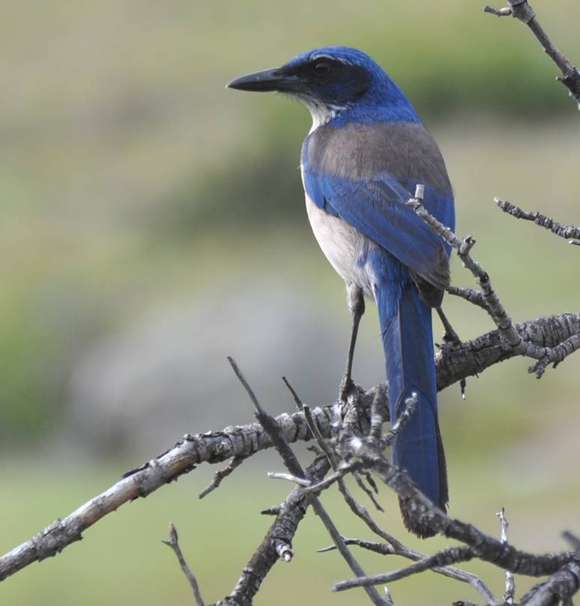
\includegraphics[width=0.5\textwidth]{../../lectures/modeling-intro/figs/issj}
    The Island Scrub-Jay
  \end{center}
\end{frame}



\begin{frame}[plain]
  \frametitle{Example}
  \Huge
  \begin{center}
    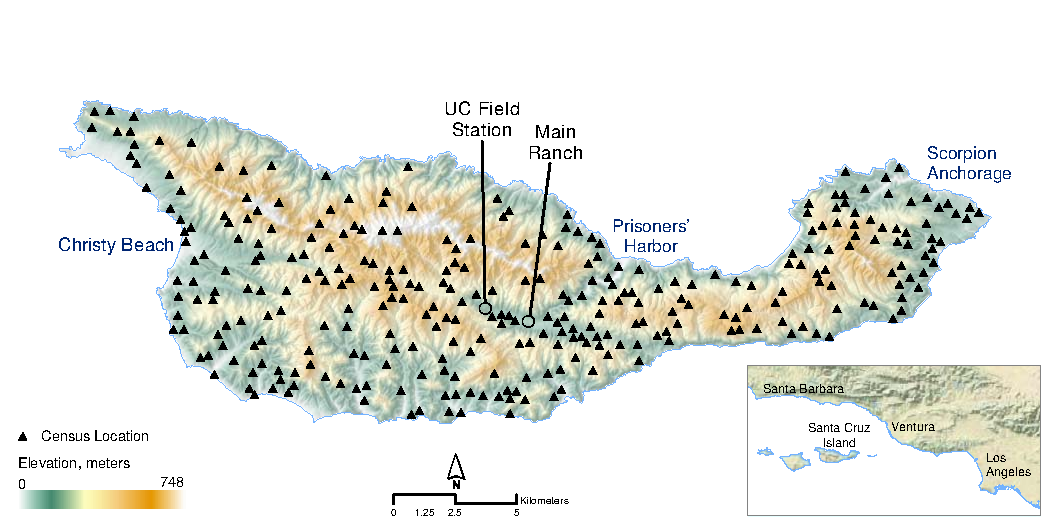
\includegraphics[width=0.8\textwidth]{../../lectures/modeling-intro/figs/Santa-Cruz} \\
    Santa Cruz Island
  \end{center}
\end{frame}




\begin{frame}[fragile]
  \frametitle{Santa Cruz Data}
  \footnotesize
%<<echo=false>>=
%##library(unmarked)
%##head(cruz)
%@
%<<echo=false,results=hide>>=
%cruzData <- cruz
%set.seed(43893)
%<<>>=
%cruzData$habitat <- factor(sample(c("Pine","Oak","Bare"),
%                               size=nrow(cruzData), replace=TRUE,
%                               prob=c(0.3, 0.6, 0.1)))
%cruzData$seeds <- factor(sample(c("Low","Med","High"),
%                               size=nrow(cruzData), replace=TRUE,
%                               prob=c(0.3, 0.6, 0.1)))
%@
%plots <- sample(1:nrow(cruzData), size=100)
%jayData <- cruzData[plots,]
%jayX <- model.matrix(~elevation+I(elevation^2)+chaparral+habitat, jayData)
%jayBeta <- c(30, 0.01, -0.000001, 1, 2.5, 1.5)
%summary(jaymu <- jayX %*% jayBeta)
%sigmaSq <- 5
%set.seed(4530)
%summary(jayData$jays <- round(rnorm(nrow(jayData), jaymu, sqrt(sigmaSq))))
%# hist(jayData$jays)
%summary(lm(jays ~ elevation + I(elevation^2) + chaparral + habitat + forest + seeds,
%           jayData))
%@
%\pause
%{\bf Add 2 fake variables}
%<<>>=
%head(cruzData)
%@
\begin{knitrout}
\definecolor{shadecolor}{rgb}{0.878, 0.918, 0.933}\color{fgcolor}\begin{kframe}
\begin{alltt}
\hlstd{cruzData} \hlkwb{<-} \hlkwd{read.csv}\hlstd{(}\hlstr{"cruzData.csv"}\hlstd{)}
\hlkwd{head}\hlstd{(cruzData,} \hlkwc{n}\hlstd{=}\hlnum{7}\hlstd{)}
\end{alltt}
\begin{verbatim}
##          x       y elevation forest chaparral habitat seeds
## 1 230736.7 3774324       241      0         0     Oak   Low
## 2 231036.7 3774324       323      0         0    Pine   Med
## 3 231336.7 3774324       277      0         0    Pine  High
## 4 230436.7 3774024        13      0         0     Oak   Med
## 5 230736.7 3774024       590      0         0     Oak  High
## 6 231036.7 3774024       533      0         0     Oak   Low
## 7 231336.7 3774024       378      0         0     Oak   Low
\end{verbatim}
\end{kframe}
\end{knitrout}
  {Each row of this data frame corresponds to a grid cell. There are 2787 grid cells covering the island. \\} 
\end{frame}



\begin{frame}[fragile]
  \frametitle{Maps of predictor variables}
%  {\bf Elevation}
  \scriptsize
%% <<elevJay,include=TRUE,fig.width=6,fig.height=4,size='scriptsize'>>=
\begin{knitrout}\scriptsize
\definecolor{shadecolor}{rgb}{0.878, 0.918, 0.933}\color{fgcolor}\begin{kframe}
\begin{alltt}
\hlkwd{library}\hlstd{(lattice)}
\hlkwd{levelplot}\hlstd{(elevation} \hlopt{~} \hlstd{x} \hlopt{+} \hlstd{y,} \hlkwc{data}\hlstd{=cruzData,}
          \hlkwc{aspect}\hlstd{=}\hlstr{"iso"}\hlstd{,} \hlcom{# Puts x and y axes on same scale}
          \hlkwc{xlab}\hlstd{=}\hlstr{"Easting"}\hlstd{,} \hlkwc{ylab}\hlstd{=}\hlstr{"Northing"}\hlstd{,} \hlkwc{main}\hlstd{=}\hlstr{"Elevation"}\hlstd{)}
\end{alltt}
\end{kframe}
\includegraphics[width=\maxwidth]{figure/elevJay-1} 

\end{knitrout}
\centering
\includegraphics[width=0.8\textwidth]{figure/elevJay-1} \\
%{This ``raster'' image is the grid. Each grid cell has multiple
%  predictor variables associated with it. \\}
\end{frame}




\begin{frame}[fragile]
  \frametitle{Maps of predictor variables}
%  {\bf Forest cover}
  \scriptsize
%% <<forestJay,include=FALSE,fig.width=6,fig.height=4>>=
\begin{knitrout}\scriptsize
\definecolor{shadecolor}{rgb}{0.878, 0.918, 0.933}\color{fgcolor}\begin{kframe}
\begin{alltt}
\hlkwd{levelplot}\hlstd{(forest} \hlopt{~} \hlstd{x} \hlopt{+} \hlstd{y,} \hlkwc{data}\hlstd{=cruzData,} \hlkwc{aspect}\hlstd{=}\hlstr{"iso"}\hlstd{,}
          \hlkwc{xlab}\hlstd{=}\hlstr{""}\hlstd{,}\hlkwc{ylab}\hlstd{=}\hlstr{""}\hlstd{,}\hlkwc{main}\hlstd{=}\hlstr{"Forest Cover"}\hlstd{,}
          \hlkwc{scales}\hlstd{=}\hlkwd{list}\hlstd{(}\hlkwc{draw}\hlstd{=}\hlnum{FALSE}\hlstd{))} \hlcom{# suppress axes}
\end{alltt}
\end{kframe}
\includegraphics[width=\maxwidth]{figure/forestJay-1} 

\end{knitrout}
\centering
\includegraphics[width=0.8\textwidth]{figure/forestJay-1} \\
\end{frame}



\begin{comment}
\begin{frame}[fragile]
  \frametitle{Maps of predictor variables}
%  {\bf Habitat type}
  \scriptsize
%% <<habitat,include=FALSE,fig.width=6,fig.height=4>>=
\begin{knitrout}\scriptsize
\definecolor{shadecolor}{rgb}{0.878, 0.918, 0.933}\color{fgcolor}\begin{kframe}
\begin{alltt}
\hlkwd{levelplot}\hlstd{(habitat} \hlopt{~} \hlstd{x} \hlopt{+} \hlstd{y,} \hlkwc{data}\hlstd{=cruzData,} \hlkwc{aspect}\hlstd{=}\hlstr{"iso"}\hlstd{,}
          \hlkwc{xlab}\hlstd{=}\hlstr{""}\hlstd{,} \hlkwc{ylab}\hlstd{=}\hlstr{""}\hlstd{,} \hlkwc{main}\hlstd{=}\hlstr{"Habitat type"}\hlstd{,}
          \hlkwc{scales}\hlstd{=}\hlkwd{list}\hlstd{(}\hlkwc{draw}\hlstd{=}\hlnum{FALSE}\hlstd{))}
\end{alltt}
\end{kframe}
\includegraphics[width=\maxwidth]{figure/habitat-1} 

\end{knitrout}
\includegraphics[width=\textwidth]{figure/habitat-1} \\
{This habitat layer is obviously fake.}
\end{frame}
\end{comment}



\begin{comment}
\begin{frame}
  \frametitle{Questions}
  \Large
%  \begin{enumerate}[<+- | visible@+->][\bf \color{PineGreen} (1)]
  \begin{enumerate}[\bf \color{PineGreen} (1)]
    \item How many jays are on the island?
    \item Where is abundance highest?
%    \item In which habitat is abundance highest?
    \item What variables are correlated with abundance?
%    \item Can we predict the consequences of environmental change?
  \end{enumerate}
\end{frame}
\end{comment}





\begin{frame}[fragile]
  \frametitle{The (fake) jay data}
  \footnotesize
\begin{knitrout}\scriptsize
\definecolor{shadecolor}{rgb}{0.878, 0.918, 0.933}\color{fgcolor}\begin{kframe}
\begin{alltt}
\hlkwd{library}\hlstd{(latticeExtra)} \hlcom{## install.packages("latticeExtra") ## Do this!}
\hlstd{jayData} \hlkwb{<-} \hlkwd{read.csv}\hlstd{(}\hlstr{"jayData.csv"}\hlstd{)}
\hlkwd{head}\hlstd{(jayData)}
\end{alltt}
\begin{verbatim}
##          x       y elevation forest chaparral habitat seeds jays
## 1 258636.7 3764124       423   0.00      0.02     Oak   Med   34
## 2 261936.7 3769224       506   0.10      0.45     Oak   Med   38
## 3 246336.7 3764124       859   0.00      0.26     Oak  High   40
## 4 239436.7 3763524      1508   0.02      0.03    Pine   Med   43
## 5 239436.7 3767724       483   0.26      0.37     Oak   Med   36
## 6 236436.7 3769524       830   0.00      0.01     Oak   Low   39
\end{verbatim}
\end{kframe}
\end{knitrout}
\begin{knitrout}\scriptsize
\definecolor{shadecolor}{rgb}{0.878, 0.918, 0.933}\color{fgcolor}\begin{kframe}
\begin{alltt}
\hlkwd{str}\hlstd{(jayData)} \hlcom{## 100 rows}
\end{alltt}
\begin{verbatim}
## 'data.frame':	100 obs. of  8 variables:
##  $ x        : num  258637 261937 246337 239437 239437 ...
##  $ y        : num  3764124 3769224 3764124 3763524 3767724 ...
##  $ elevation: int  423 506 859 1508 483 830 457 304 834 164 ...
##  $ forest   : num  0 0.1 0 0.02 0.26 0 0.02 0 0.54 0 ...
##  $ chaparral: num  0.02 0.45 0.26 0.03 0.37 0.01 0.22 0.09 0.21 0.11 ...
##  $ habitat  : Factor w/ 3 levels "Bare","Oak","Pine": 2 2 2 3 2 2 2 3 3 3 ...
##  $ seeds    : Factor w/ 3 levels "High","Low","Med": 3 3 1 3 3 2 3 2 3 1 ...
##  $ jays     : int  34 38 40 43 36 39 38 35 41 33 ...
\end{verbatim}
\end{kframe}
\end{knitrout}
\end{frame}




\begin{frame}[fragile]
  \frametitle{Maps of predictor variables}
\begin{knitrout}\scriptsize
\definecolor{shadecolor}{rgb}{0.878, 0.918, 0.933}\color{fgcolor}\begin{kframe}
\begin{alltt}
\hlkwd{levelplot}\hlstd{(chaparral} \hlopt{~} \hlstd{x} \hlopt{+} \hlstd{y,} \hlkwc{data}\hlstd{=cruzData,} \hlkwc{aspect}\hlstd{=}\hlstr{"iso"}\hlstd{,}
          \hlkwc{xlab}\hlstd{=}\hlstr{""}\hlstd{,} \hlkwc{ylab}\hlstd{=}\hlstr{""}\hlstd{,} \hlkwc{main}\hlstd{=}\hlstr{"Chaparral and survey plots"}\hlstd{,}
          \hlkwc{scales}\hlstd{=}\hlkwd{list}\hlstd{(}\hlkwc{draw}\hlstd{=}\hlnum{FALSE}\hlstd{))} \hlopt{+}
    \hlkwd{xyplot}\hlstd{(y} \hlopt{~} \hlstd{x, jayData,} \hlkwc{pch}\hlstd{=}\hlnum{0}\hlstd{,} \hlkwc{col}\hlstd{=}\hlnum{1}\hlstd{,} \hlkwc{cex}\hlstd{=}\hlnum{0.5}\hlstd{)}
\end{alltt}
\end{kframe}
\end{knitrout}
%\vspace{-2cm}
\footnotesize
\centering
\includegraphics[width=0.9\textwidth]{figure/plots-1} \\
Jays were surveyed at this subset of 100 grid cells \\
\end{frame}



\begin{frame}[fragile]
  \frametitle{Fit some models -- Simple linear regression}
%  {\bf Simple linear regression}
  \scriptsize
\begin{knitrout}
\definecolor{shadecolor}{rgb}{0.878, 0.918, 0.933}\color{fgcolor}\begin{kframe}
\begin{alltt}
\hlstd{fm1} \hlkwb{<-} \hlkwd{lm}\hlstd{(jays} \hlopt{~} \hlstd{elevation,} \hlkwc{data}\hlstd{=jayData)}
\end{alltt}
\end{kframe}
\end{knitrout}
\pause
\begin{knitrout}
\definecolor{shadecolor}{rgb}{0.878, 0.918, 0.933}\color{fgcolor}\begin{kframe}
\begin{alltt}
\hlkwd{summary}\hlstd{(fm1)}
\end{alltt}
\begin{verbatim}
## 
## Call:
## lm(formula = jays ~ elevation, data = jayData)
## 
## Residuals:
##     Min      1Q  Median      3Q     Max 
## -5.4874 -1.7539  0.1566  1.6159  4.6155 
## 
## Coefficients:
##              Estimate Std. Error t value Pr(>|t|)    
## (Intercept) 33.082808   0.453997   72.87   <2e-16 ***
## elevation    0.008337   0.000595   14.01   <2e-16 ***
## ---
## Signif. codes:  0 '***' 0.001 '**' 0.01 '*' 0.05 '.' 0.1 ' ' 1
## 
## Residual standard error: 2.285 on 98 degrees of freedom
## Multiple R-squared:  0.667,	Adjusted R-squared:  0.6636 
## F-statistic: 196.3 on 1 and 98 DF,  p-value: < 2.2e-16
\end{verbatim}
\end{kframe}
\end{knitrout}
\end{frame}




\begin{frame}[fragile]
  \frametitle{\normalsize Fit some models -- Linear regression with quadratic effects}
%  {\bf Linear regression with quadratic term}
  \scriptsize
\begin{knitrout}\scriptsize
\definecolor{shadecolor}{rgb}{0.878, 0.918, 0.933}\color{fgcolor}\begin{kframe}
\begin{alltt}
\hlstd{fm2} \hlkwb{<-} \hlkwd{lm}\hlstd{(jays} \hlopt{~} \hlstd{elevation} \hlopt{+} \hlkwd{I}\hlstd{(elevation}\hlopt{^}\hlnum{2}\hlstd{),} \hlkwc{data}\hlstd{=jayData)}
\end{alltt}
\end{kframe}
\end{knitrout}
\pause
\begin{knitrout}\scriptsize
\definecolor{shadecolor}{rgb}{0.878, 0.918, 0.933}\color{fgcolor}\begin{kframe}
\begin{alltt}
\hlkwd{summary}\hlstd{(fm2)}
\end{alltt}
\begin{verbatim}
## 
## Call:
## lm(formula = jays ~ elevation + I(elevation^2), data = jayData)
## 
## Residuals:
##     Min      1Q  Median      3Q     Max 
## -4.8429 -1.4608  0.1304  1.5908  4.7854 
## 
## Coefficients:
##                  Estimate Std. Error t value Pr(>|t|)    
## (Intercept)     3.162e+01  7.631e-01  41.434  < 2e-16 ***
## elevation       1.368e-02  2.342e-03   5.843 6.86e-08 ***
## I(elevation^2) -3.542e-06  1.503e-06  -2.357   0.0204 *  
## ---
## Signif. codes:  0 '***' 0.001 '**' 0.01 '*' 0.05 '.' 0.1 ' ' 1
## 
## Residual standard error: 2.233 on 97 degrees of freedom
## Multiple R-squared:  0.6851,	Adjusted R-squared:  0.6786 
## F-statistic: 105.5 on 2 and 97 DF,  p-value: < 2.2e-16
\end{verbatim}
\end{kframe}
\end{knitrout}
\end{frame}





\begin{frame}[fragile]
  \frametitle{Fit some models -- Multiple linear regression}
%  {\bf Multiple linear regression}
  \scriptsize
\begin{knitrout}\scriptsize
\definecolor{shadecolor}{rgb}{0.878, 0.918, 0.933}\color{fgcolor}\begin{kframe}
\begin{alltt}
\hlstd{fm3} \hlkwb{<-} \hlkwd{lm}\hlstd{(jays} \hlopt{~} \hlstd{elevation} \hlopt{+} \hlstd{chaparral,} \hlkwc{data}\hlstd{=jayData)}
\end{alltt}
\end{kframe}
\end{knitrout}
\pause
\begin{knitrout}\scriptsize
\definecolor{shadecolor}{rgb}{0.878, 0.918, 0.933}\color{fgcolor}\begin{kframe}
\begin{alltt}
\hlkwd{summary}\hlstd{(fm3)}
\end{alltt}
\begin{verbatim}
## 
## Call:
## lm(formula = jays ~ elevation + chaparral, data = jayData)
## 
## Residuals:
##     Min      1Q  Median      3Q     Max 
## -5.1584 -1.5779  0.0226  1.5315  4.6003 
## 
## Coefficients:
##              Estimate Std. Error t value Pr(>|t|)    
## (Intercept) 3.284e+01  4.982e-01  65.919   <2e-16 ***
## elevation   8.224e-03  6.017e-04  13.669   <2e-16 ***
## chaparral   1.308e+00  1.124e+00   1.163    0.248    
## ---
## Signif. codes:  0 '***' 0.001 '**' 0.01 '*' 0.05 '.' 0.1 ' ' 1
## 
## Residual standard error: 2.281 on 97 degrees of freedom
## Multiple R-squared:  0.6716,	Adjusted R-squared:  0.6649 
## F-statistic:  99.2 on 2 and 97 DF,  p-value: < 2.2e-16
\end{verbatim}
\end{kframe}
\end{knitrout}
\end{frame}





\begin{frame}[fragile]
  \frametitle{Fit some models -- One-way ANOVA}
%  {\bf One-way ANOVA}
  \scriptsize
\begin{knitrout}\scriptsize
\definecolor{shadecolor}{rgb}{0.878, 0.918, 0.933}\color{fgcolor}\begin{kframe}
\begin{alltt}
\hlstd{fm4} \hlkwb{<-} \hlkwd{lm}\hlstd{(jays} \hlopt{~} \hlstd{habitat,} \hlkwc{data}\hlstd{=jayData)}
\end{alltt}
\end{kframe}
\end{knitrout}
\pause
\begin{knitrout}\scriptsize
\definecolor{shadecolor}{rgb}{0.878, 0.918, 0.933}\color{fgcolor}\begin{kframe}
\begin{alltt}
\hlkwd{summary}\hlstd{(fm4)}
\end{alltt}
\begin{verbatim}
## 
## Call:
## lm(formula = jays ~ habitat, data = jayData)
## 
## Residuals:
##     Min      1Q  Median      3Q     Max 
## -7.9143 -2.3684 -0.3684  3.0857  8.6316 
## 
## Coefficients:
##             Estimate Std. Error t value Pr(>|t|)    
## (Intercept)   35.875      1.356  26.456   <2e-16 ***
## habitatOak     3.493      1.448   2.413   0.0177 *  
## habitatPine    2.039      1.503   1.357   0.1780    
## ---
## Signif. codes:  0 '***' 0.001 '**' 0.01 '*' 0.05 '.' 0.1 ' ' 1
## 
## Residual standard error: 3.835 on 97 degrees of freedom
## Multiple R-squared:  0.07126,	Adjusted R-squared:  0.05211 
## F-statistic: 3.721 on 2 and 97 DF,  p-value: 0.02773
\end{verbatim}
\end{kframe}
\end{knitrout}
\end{frame}



\begin{frame}[fragile]
  \frametitle{Fit some models -- ANCOVA}
%  {\bf ANCOVA}
%  \tiny
\begin{knitrout}\scriptsize
\definecolor{shadecolor}{rgb}{0.878, 0.918, 0.933}\color{fgcolor}\begin{kframe}
\begin{alltt}
\hlstd{fm5} \hlkwb{<-} \hlkwd{lm}\hlstd{(jays} \hlopt{~} \hlstd{habitat} \hlopt{+} \hlstd{elevation,} \hlkwc{data}\hlstd{=jayData)}
\hlkwd{summary}\hlstd{(fm5)}
\end{alltt}
\begin{verbatim}
## 
## Call:
## lm(formula = jays ~ habitat + elevation, data = jayData)
## 
## Residuals:
##     Min      1Q  Median      3Q     Max 
## -5.0327 -1.5356  0.0091  1.4686  4.2391 
## 
## Coefficients:
##              Estimate Std. Error t value Pr(>|t|)    
## (Intercept) 3.072e+01  8.084e-01  37.997  < 2e-16 ***
## habitatOak  3.166e+00  7.850e-01   4.034  0.00011 ***
## habitatPine 1.695e+00  8.148e-01   2.081  0.04010 *  
## elevation   8.289e-03  5.414e-04  15.308  < 2e-16 ***
## ---
## Signif. codes:  0 '***' 0.001 '**' 0.01 '*' 0.05 '.' 0.1 ' ' 1
## 
## Residual standard error: 2.078 on 96 degrees of freedom
## Multiple R-squared:  0.7301,	Adjusted R-squared:  0.7217 
## F-statistic: 86.56 on 3 and 96 DF,  p-value: < 2.2e-16
\end{verbatim}
\end{kframe}
\end{knitrout}
\end{frame}




\begin{frame}[fragile]
  \frametitle{\small One factor and continuous covariates with quadratic effects}
%  {\small \bf Factor and two continuous covariates, one with quadratic effects}
  \tiny
\begin{knitrout}\scriptsize
\definecolor{shadecolor}{rgb}{0.878, 0.918, 0.933}\color{fgcolor}\begin{kframe}
\begin{alltt}
\hlstd{fm6} \hlkwb{<-} \hlkwd{lm}\hlstd{(jays} \hlopt{~} \hlstd{habitat} \hlopt{+} \hlstd{elevation} \hlopt{+}
          \hlkwd{I}\hlstd{(elevation}\hlopt{^}\hlnum{2}\hlstd{)} \hlopt{+} \hlstd{chaparral,} \hlkwc{data}\hlstd{=jayData)}
\hlkwd{summary}\hlstd{(fm6)}
\end{alltt}
\begin{verbatim}
## 
## Call:
## lm(formula = jays ~ habitat + elevation + I(elevation^2) + chaparral, 
##     data = jayData)
## 
## Residuals:
##     Min      1Q  Median      3Q     Max 
## -5.3162 -1.4301  0.0168  1.3802  4.0673 
## 
## Coefficients:
##                  Estimate Std. Error t value Pr(>|t|)    
## (Intercept)     2.958e+01  9.988e-01  29.610  < 2e-16 ***
## habitatOak      3.071e+00  7.788e-01   3.943 0.000155 ***
## habitatPine     1.802e+00  8.106e-01   2.223 0.028643 *  
## elevation       1.192e-02  2.254e-03   5.291 7.93e-07 ***
## I(elevation^2) -2.453e-06  1.441e-06  -1.702 0.092075 .  
## chaparral       7.886e-01  1.026e+00   0.768 0.444177    
## ---
## Signif. codes:  0 '***' 0.001 '**' 0.01 '*' 0.05 '.' 0.1 ' ' 1
## 
## Residual standard error: 2.058 on 94 degrees of freedom
## Multiple R-squared:  0.7409,	Adjusted R-squared:  0.7272 
## F-statistic: 53.77 on 5 and 94 DF,  p-value: < 2.2e-16
\end{verbatim}
\end{kframe}
\end{knitrout}
\end{frame}




\begin{frame}[fragile]
  \frametitle{Visualize the quadratic effect}
  {\small
    Create a sequence of values of elevation, holding other predictors
    constant \\}  
  \footnotesize
\begin{knitrout}\footnotesize
\definecolor{shadecolor}{rgb}{0.878, 0.918, 0.933}\color{fgcolor}\begin{kframe}
\begin{alltt}
\hlstd{nd1} \hlkwb{<-} \hlkwd{data.frame}\hlstd{(}\hlkwc{habitat} \hlstd{=} \hlstr{"Oak"}\hlstd{,}
    \hlkwc{elevation}\hlstd{=}\hlkwd{seq}\hlstd{(}\hlkwd{min}\hlstd{(jayData}\hlopt{$}\hlstd{elev),} \hlkwd{max}\hlstd{(jayData}\hlopt{$}\hlstd{elev),} \hlkwc{length}\hlstd{=}\hlnum{100}\hlstd{),}
    \hlkwc{chaparral}\hlstd{=}\hlkwd{mean}\hlstd{(jayData}\hlopt{$}\hlstd{chaparral))}
\end{alltt}
\end{kframe}
\end{knitrout}
\pause
\vfill
  \small
{\small Obtain the predictions}
\footnotesize
\begin{knitrout}\footnotesize
\definecolor{shadecolor}{rgb}{0.878, 0.918, 0.933}\color{fgcolor}\begin{kframe}
\begin{alltt}
\hlstd{E6.elev} \hlkwb{<-} \hlkwd{predict}\hlstd{(fm6,} \hlkwc{newdata}\hlstd{=nd1,} \hlkwc{type}\hlstd{=}\hlstr{"response"}\hlstd{,} \hlkwc{se.fit}\hlstd{=}\hlnum{TRUE}\hlstd{,}
                   \hlkwc{interval}\hlstd{=}\hlstr{"confidence"}\hlstd{)}
\hlstd{E6.elev} \hlkwb{<-} \hlkwd{cbind}\hlstd{(E6.elev}\hlopt{$}\hlstd{fit, nd1)}
\hlkwd{head}\hlstd{(E6.elev)}
\end{alltt}
\begin{verbatim}
##        fit      lwr      upr habitat elevation chaparral
## 1 32.97879 31.46749 34.49009     Oak  12.00000    0.2407
## 2 33.16096 31.70991 34.61202     Oak  27.40404    0.2407
## 3 33.34197 31.94945 34.73449     Oak  42.80808    0.2407
## 4 33.52181 32.18609 34.85754     Oak  58.21212    0.2407
## 5 33.70049 32.41978 34.98120     Oak  73.61616    0.2407
## 6 33.87801 32.65051 35.10551     Oak  89.02020    0.2407
\end{verbatim}
\end{kframe}
\end{knitrout}
\end{frame}





\begin{frame}[fragile]
  \frametitle{Visualize the quadratic effect}
%  \tiny
\begin{knitrout}\scriptsize
\definecolor{shadecolor}{rgb}{0.878, 0.918, 0.933}\color{fgcolor}\begin{kframe}
\begin{alltt}
\hlkwd{plot}\hlstd{(fit} \hlopt{~} \hlstd{elevation, E6.elev,} \hlkwc{type}\hlstd{=}\hlstr{"l"}\hlstd{,} \hlkwc{ylim}\hlstd{=}\hlkwd{c}\hlstd{(}\hlnum{20}\hlstd{,}\hlnum{50}\hlstd{),}
     \hlkwc{xlab}\hlstd{=}\hlstr{"Elevation (m)"}\hlstd{,} \hlkwc{ylab}\hlstd{=}\hlstr{"Expected number of jays"}\hlstd{)}
\hlkwd{points}\hlstd{(jays} \hlopt{~} \hlstd{elevation, jayData)}
\hlkwd{lines}\hlstd{(lwr} \hlopt{~} \hlstd{elevation, E6.elev,} \hlkwc{lty}\hlstd{=}\hlnum{2}\hlstd{)}
\hlkwd{lines}\hlstd{(upr} \hlopt{~} \hlstd{elevation, E6.elev,} \hlkwc{lty}\hlstd{=}\hlnum{2}\hlstd{)}
\end{alltt}
\end{kframe}
\end{knitrout}
\centering
\includegraphics[width=0.8\textwidth]{figure/E6elev-1} \\
\end{frame}






\begin{frame}[fragile]
  \frametitle{\normalsize Predict jay abundance at each pixel on Santa Cruz}
  \scriptsize
\begin{knitrout}
\definecolor{shadecolor}{rgb}{0.878, 0.918, 0.933}\color{fgcolor}\begin{kframe}
\begin{alltt}
\hlstd{E6} \hlkwb{<-} \hlkwd{predict}\hlstd{(fm6,} \hlkwc{type}\hlstd{=}\hlstr{"response"}\hlstd{,} \hlkwc{newdata}\hlstd{=cruzData,} \hlkwc{interval}\hlstd{=}\hlstr{"confidence"}\hlstd{)}
\end{alltt}
\end{kframe}
\end{knitrout}
\pause
\begin{knitrout}
\definecolor{shadecolor}{rgb}{0.878, 0.918, 0.933}\color{fgcolor}\begin{kframe}
\begin{alltt}
\hlstd{E6} \hlkwb{<-} \hlkwd{cbind}\hlstd{(cruzData[,}\hlkwd{c}\hlstd{(}\hlstr{"x"}\hlstd{,}\hlstr{"y"}\hlstd{)], E6)}
\hlkwd{head}\hlstd{(E6,} \hlkwc{n}\hlstd{=}\hlnum{4}\hlstd{)}
\end{alltt}
\begin{verbatim}
##          x       y      fit      lwr      upr
## 1 230736.7 3774324 35.37722 34.48977 36.26466
## 2 231036.7 3774324 34.97211 34.08259 35.86163
## 3 231336.7 3774324 34.49135 33.59102 35.39168
## 4 230436.7 3774024 32.80085 31.29979 34.30191
\end{verbatim}
\end{kframe}
\end{knitrout}
\pause
{\bf Another way to obtain the predictions:}
\begin{knitrout}
\definecolor{shadecolor}{rgb}{0.878, 0.918, 0.933}\color{fgcolor}\begin{kframe}
\begin{alltt}
\hlstd{X} \hlkwb{<-} \hlkwd{model.matrix}\hlstd{(}\hlopt{~}\hlstd{habitat}\hlopt{+}\hlstd{elevation}\hlopt{+}\hlkwd{I}\hlstd{(elevation}\hlopt{^}\hlnum{2}\hlstd{)}\hlopt{+}
                  \hlstd{chaparral,} \hlkwc{data}\hlstd{=cruzData)}
\hlstd{beta} \hlkwb{<-} \hlkwd{coef}\hlstd{(fm6)} \hlcom{# beta estimates}
\hlstd{E} \hlkwb{<-} \hlstd{X} \hlopt \hlstd{beta}   \hlcom{# expected number of jays at each pixel}
\hlkwd{head}\hlstd{(E,} \hlkwc{n}\hlstd{=}\hlnum{4}\hlstd{)}
\end{alltt}
\begin{verbatim}
##       [,1]
## 1 35.37722
## 2 34.97211
## 3 34.49135
## 4 32.80085
\end{verbatim}
\end{kframe}
\end{knitrout}
\end{frame}


\begin{frame}[fragile]
  \frametitle{Map the predictions}
  \scriptsize

\includegraphics[width=\textwidth]{figure/Ejay-1}
\end{frame}




\begin{frame}[fragile]
  \frametitle{Map the predictions}
  \scriptsize

\includegraphics[width=\textwidth]{figure/Ljay-1}
\end{frame}




\begin{frame}[fragile]
  \frametitle{Map the predictions}
  \scriptsize

\includegraphics[width=\textwidth]{figure/Ujay-1}
\end{frame}




%% \begin{frame}[fragile]
%%   \frametitle{Future scenarios}
%%   {\bf What if the pine and oak disappear? \par}
%%   \pause
%%   \vspace{0.3cm}
%%   {\bf \dots assuming {\tt fm5} is the {\it correct} model}
%%   \pause
%%   \vspace{0.3cm}
%%   \footnotesize
%% <<>>=
%% future1 <- cruzData
%% future1$habitat[] <- "Bare"
%% future.pred1 <- predict(fm5, type="response", newdata=future1,
%%                         interval="confidence")
%% future.pred1 <- cbind(cruzData[,c("x","y")], future.pred1)
%% @
%% \end{frame}



%% \begin{frame}[fragile]
%%   \frametitle{Future with no oak or pine}
%%   \scriptsize
%% <<future1,include=FALSE,fig.width=6,fig.height=4>>=
%% levelplot(fit ~ x + y, data=future.pred1, aspect="iso",
%%           xlab="", ylab="", main="Expected values",
%%           at=25:55, colorkey=list(space="bottom"),
%%           scales=list(draw=FALSE))
%% @
%% \includegraphics[width=\textwidth]{lab12-modeling-future1}
%% \end{frame}





%% \begin{frame}[fragile]
%%   \frametitle{Future scenarios}
%%   {\bf What if the island sinks 1000 m? \par}
%%   \vspace{0.3cm}
%% %  \pause
%% %  {\bf \dots assuming {\tt fm5} is the {\it correct} model}
%%   \pause
%%   \footnotesize
%% <<>>=
%% future2 <- cruzData
%% future2$elevation <- future2$elevation - 1000
%% future2$elevation[future2$elevation < 0] <- NA
%% future.pred2 <- predict(fm5, type="response", newdata=future2,
%%                         interval="confidence")
%% future.pred2 <- cbind(cruzData[,c("x","y")], future.pred2)
%% @
%% \end{frame}




%% \begin{frame}[fragile]
%%   \frametitle{The island sinks 1000 m}
%%   \scriptsize
%% <<future2,echo=false,include=FALSE,fig.width=6,fig.height=4>>=
%% levelplot(fit ~ x + y, data=future.pred2, aspect="iso",
%%           panel = function(...) {
%%               panel.fill(col="skyblue1")
%%               panel.levelplot(...)
%%           },
%%           xlab="", ylab="", main="Expected values",
%%           at=25:55, colorkey=list(space="bottom"),
%%           scales=list(draw=FALSE))
%% @
%% \includegraphics[width=\textwidth]{lab12-modeling-future2}
%% \end{frame}













\section{Switzerland Assignment}




\begin{frame}
  \centering \Huge \color{blue}{Assignment} \par
\end{frame}



\begin{frame}[fragile]
  \frametitle{Species Richness in Switzerland}
  \large
%  \begin{itemize}%[<+->]
%    \item
  Birds are sampled at 267 locations (quadrats) as part of the
  Swiss breeding bird survey \\
  \vfill
%    \item
  The following predictor variables are available: elevation,
      percent cover of forest, and the presence of water \\
  \vfill
%    \item
  The country-wide data are in the file {\tt Switzerland.csv} \\
%    \item
  \vfill
  The species richness data for the 267 quadrats are in the
      file {\tt swissBirds.csv}
%  \end{itemize}
\end{frame}




\begin{frame}[fragile]
  \frametitle{Switzerland}
  \tiny

\includegraphics[width=\textwidth]{figure/elev-1}
\end{frame}



\begin{frame}[fragile]
  \frametitle{Switzerland}
  \tiny

\includegraphics[width=\textwidth]{figure/forest-1}
\end{frame}





\begin{frame}[fragile]
  \frametitle{Switzerland}
  \tiny

\includegraphics[width=\textwidth]{figure/water-1}
\end{frame}

%\end{document}


\begin{frame}[fragile]
%summary(lm(sppRichness ~ forest + I(forest^2) + elevation * water, data=swissData))
%#levelplot(I(43.24 + 0.317*forest + -0.00109*forest^2 + -0.009132*elevation) ~ x + y,
%#          data=Switzerland, aspect="iso")
%@
\begin{knitrout}
\definecolor{shadecolor}{rgb}{0.878, 0.918, 0.933}\color{fgcolor}\begin{kframe}
\begin{alltt}
\hlstd{swissData} \hlkwb{<-} \hlkwd{read.csv}\hlstd{(}\hlstr{"swissData.csv"}\hlstd{)}
\hlkwd{head}\hlstd{(swissData,} \hlkwc{n}\hlstd{=}\hlnum{7}\hlstd{)}
\end{alltt}
\begin{verbatim}
##   elevation forest water sppRichness
## 1       450      3    No          35
## 2       450     21    No          51
## 3      1050     32    No          46
## 4       950      9   Yes          31
## 5      1150     35   Yes          50
## 6       550      2    No          43
## 7       750      6    No          37
\end{verbatim}
\end{kframe}
\end{knitrout}
\end{frame}





\begin{frame}
  \frametitle{Assignment}
  \large
  {\bf Create an \R~script to do the following}
%  \pause
%  \begin{enumerate}[<+- | visible@+->][\bf \color{PineGreen} (1)]
  \begin{enumerate}[\bf \color{PineGreen} (1)]
    \item Fit 4 models of species richness using {\tt lm}.
      \begin{itemize} \large
        \item At least one model should include an interaction, and
          one model should include quadratic effects
%        \item But make sure you can think of justification for these terms
      \end{itemize}
    \item Intepret the $\beta$ parameter estimates for each model.
    \item Create the design matrix for one of the models, and (matrix)
      multiply it by the $\beta$ coefficients. Explain what the values
      represent in the returned vector.
    %% \item Create a table with following columns:
    %%   \begin{itemize}
    %%     \item Model ID
    %%     \item Residual sum-of-squares
    %%     \item AIC
    %%     \item $\Delta$ AIC
    %%     \item Model weight $w$
    %%   \end{itemize}
    \item Use {\tt predict} to plot the relationship between expected
      species richness and the predictor variable with the quadratic
      effects. Include 95\% CI in your plot.
    \item Using the model with the interaction, predict species
      richness at each location in Switzerland. Use {\tt levelplot} to
      map the predicted values.
      %% when: forest = 25, elevation = 1000, and
      %% \begin{itemize}
      %%   \item forest = 25
      %%   \item elevation = 1000
      %%   \item water = ``No''
      %% \end{itemize}
    %% \item Create model-averaged prediction of species richness under
    %%   same conditions as above
  \end{enumerate}
\end{frame}





\end{document}

